\begin{figure}[p]
\centering
\captionsetup{justification=raggedright,labelsep=none,singlelinecheck=false,labelformat=boldlabel}
\caption[]{\footnotesize \textbf{: Gross and net Sharpe ratios for the market portfolio using pooled forecasts.} Panel A reports the long sample and Panel B the short sample. Pale bars are gross and solid bars are net of modeled factor-exposure costs. EW denotes the forecast ensemble. Each construction retains its stated exposure cap. }
\label{fig:rv-portfolio_wealth_market_pooled}
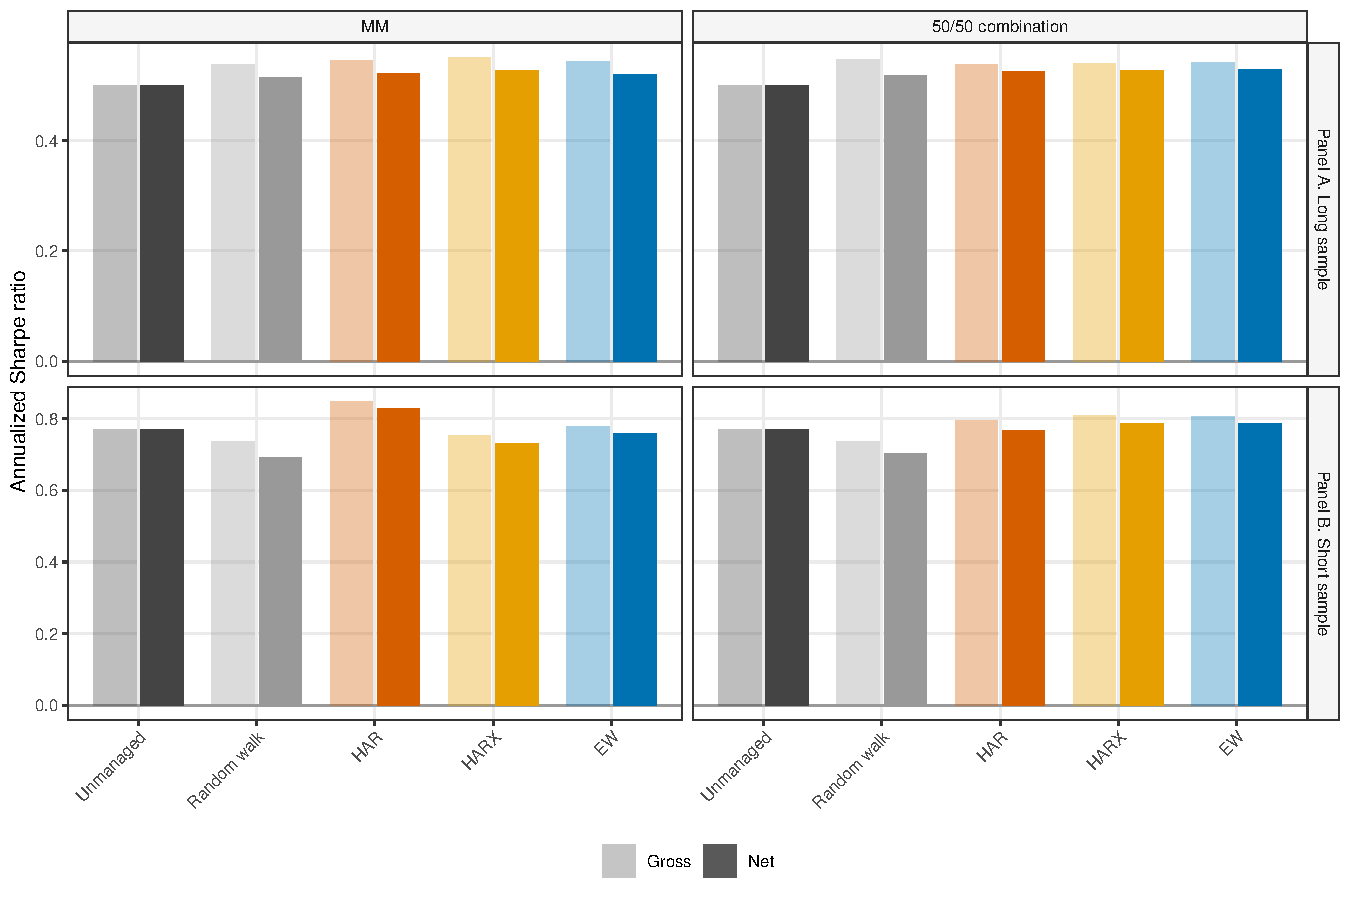
\includegraphics[width=\linewidth,height=0.70\textheight,keepaspectratio]{results_v3/combined/main_appendix/portfolio_wealth_market_pooled.pdf}
\end{figure}
